\documentclass{article}
\usepackage{graphicx} % Required for inserting images
\usepackage[top=0.9in, bottom=1in, left=1.5in, right=1.5in]{geometry}
\usepackage[utf8]{inputenc}
\usepackage[icelandic]{babel}
\usepackage[T1]{fontenc}
\usepackage[sc]{mathpazo}
\usepackage[parfill]{parskip}
\renewcommand{\baselinestretch}{1.2}
% Tables and lists
\usepackage{booktabs,tabularx}
\usepackage{multirow}
\usepackage{enumerate}
\usepackage{adjustbox}
\usepackage{multicol}
\usepackage{xcolor}
\usepackage{algpseudocode}
\usepackage{algorithm}
\usepackage{tikz}
\usepackage{nicefrac}
\usepackage{changepage}
\usepackage{fancyvrb}
\usepackage{xlop}
\usepackage{titlesec}
\titleformat{\section} 
{\normalfont\normalsize\bfseries}{Phase \thesection}{1em}{}
\usetikzlibrary{arrows, positioning, calc, graphs}

% Math
\usepackage{amsmath, amsfonts, amssymb, amsthm}
% Graphics

\usepackage{graphicx}
\usepackage{tikz}
% Code environment
\usepackage{minted}
%\usepackage{bm}
%\usepackage{siunitx}
%\usepackage{animate}
%\usepackage{hyperref}
%\usepackage{movie15}
%\usepackage{multicol}
%\usepackage{changepage}
\title{Tölvutækni og forritun Verkefni 1}
\author{Ragnar Björn Ingvarsson, rbi3}
\tikzset{->, >=stealth', shorten >=1pt, node distance=2cm,thick, main node/.style={circle,draw,minimum size=3em}}


\begin{document}
\renewcommand\thepage{}
	
	\maketitle

	\newpage
	\setcounter{page}{1}
	\renewcommand\thepage{\arabic{page}}

	\part{Verkefnislýsing}
	Í þessi verkefni eigið þið að bjarga heiminum frá hinum
	fúlmannlega doktor Vonda. Hann hefur útbúið stafrænar
	sprengjur sem þið eigið að gera óvirkar. Hver
	sprengja hefur nokkur þrep. Í hverju þrepi þurfið þið að slá
	inn tiltekinn streng (eða talnarunu) til að aftengja það þrep og
	þá færist þið yfir á næsta þrep. Ef þið sláið inn rangan streng
	þá springur sprengjan og prentar út "BOOM!!!".

	Hlutverk ykkar í þessu verkefni er að finna út hvaða strengur aftengir 
	hvert þrep og setja hann inn. Það eru 6 þrep í sprengjunni og þau 
	verða erfiðari eftir því sem lengra er komið.

	Mælt er með að nota kembiforrit eins og \textbf{gdb} og til að lesa 
	smalamálskóðann að nota \textbf{objdump}. 

	\part{Mín lausn}

	\section{}
	Ég byrjaði á að skoða phase\_1 fallið í smalamálskóðanum og tók eftir 
	í samræmi við bomb.c kóðann að strengurinn minn ætti að vera færður inn 
	í fallið sem fyrsta inntak. Ég vissi að fyrsta inntak er alltaf geymt 
	í \%rdi svo ég notaði gdb til að setja break punkt á strings\_not\_equal 
	fallið til að athuga svo gildi gista með \textbf{i r} í gdb og skoðaði 
	svo inntakið mitt í \%rdi með \textbf{x} skipuninni og formattaði 
	gildið sem streng með \textbf{x/s} og vissulega kom mitt inntak.

	Eftir það eyddi ég allt of miklum tíma í að skoða hvað 
	strings\_not\_equal fallið gerir og til að vera hreinskilinn man ég bara 
	ekkert hvað ég gerði til að finna út lausnina en ég hlýt að hafa fattað 
	að fyrst eitthvað gildi var fært inn í \%rsi fyrir kall á fallið, 
	er mjög líklegt að fallið taki þá inn tvö inntök og athugi hvort þau 
	séu eins. Þá hef ég orðið forvitinn um hvaða gildi væri sett inn í 
	\%rsi og athugað á því eins og með \%rdi. Út kemur þá 
	"Verbosity leads to unclear, inarticulate things."

	\section{}
	Það fyrsta sem ég tók eftir hér var að fallið phase\_2 kallar á fallið 
	read\_six\_numbers svo það er nokkuð augljóst þaðan að lykilorðið er 
	einhver samsetning af sex tölum. Eftir að grafa í gegn um 
	read\_six\_numbers í of langan tíma fattaði ég að fallið tekur tvö 
	inntök, fyrsta er strengur af sex tölum, semsagt bara strengurinn minn, 
	og næsta er address í minni sem tölurnar munu verða geymdar á, þar sem 
	ekki er pláss fyrir sex tölur bara í \%rax. Til að tékka á hvort þetta 
	sé satt gat ég sett break á explode\_bomb fallið og athugað gildið í 
	minni á addressinu sem \%rsp bendir á. Hér lærði ég líka að við hvert 
	kall á fall lækkar \%rsp um $8$ svo ég þarf að bæta við $8$ til að gera 
	ráð fyrir því. Eftir það er auðvelt að sjá frá kóðanum að fyrsta talan 
	er $1$ og svo er hver næsta tala eftir það með formúluna: fyrri tala + 
	index á núverandi tölu (0-indexað). Þá er næsta tala $2$, næsta $4$, svo 
	$7$, svo $11$, svo $16$. Og þar með er þetta leyst. 1 2 4 7 11 16.

	\section{}
	Hér er fyrsta skrefið að athuga að fallið \_\_isoc99\_sscanf@plt tekur 
	tvö inntök, strenginn til að lesa í \%rdi, og streng sem segir hvernig 
	á að formatta þann streng, í þessu tilfelli "\%d \%c \%d". Þá gat ég vitað að lausnin er int char int. 
Síðan tekur 
	fallið inntök fyrir staðsetningu í minni hvers gildi, svo þrjú auka í 
	þessu tilfelli, fyrsta heiltalan í rsp + 16, characterinn í rsp + 15 og 
	næsta heiltala í rsp + 20. 

	Fyrsta talan þarf svo að vera minni eða jöfn 7 svo ég ákvað að setja 7 
	sem fyrsta inntak. Nokkrir reikningar eru svo gerðir og svo kemur 
	forritið að þessari línu.

	\begin{center}
		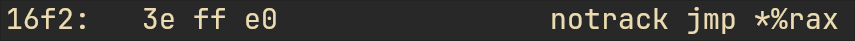
\includegraphics[scale=0.35]{notrack.png}
	\end{center}
	Ég reyndi mikið að leysa hvert forritið væri að hoppa hér með því að 
	reyna að reikna þetta sjálfur en það gekk eitthvað illa, og ég var ekki 
	búinn að læra hvernig á að breaka á sérstökum línum í gdb svo þetta var 
	smá mál. Þangað til að ég fattaði að hægt er að fara áfram þangað til 
	sprengjan springur, stoppa þar, setja "where"\hspace{.5em}inn í gdb og 
	sjá hvert explode\_bomb á að fara eftir að það er búið að keyra, og svo athuga hvaðan ég gæti hafa 
	komist þangað. Með þessu fattaði ég að ég hafði hoppað hingað

	\begin{center}
		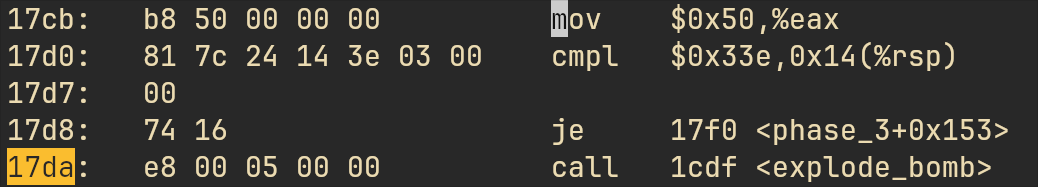
\includegraphics[scale=0.35]{jmp.png}
	\end{center}

	Og þá er einfalt að breyta hex í ascii og decimal og finna út að strengur sem 
	virkar er þá "7 P 830". (kóðinn sem athugar á char-inum er á 17f0)

	\section{}
	Hér notaði ég sömu aðferð með sscanf fallið til að sjá að inntakið ætti 
	að vera tvær heiltölur og sá svo að fyrsta inntakið mátti ekki vera 
	stærra en 14 og var svo tekið sem inntak í func4 fallið ásamt $0$ og 
	$14$. Búist er svo við gildinu 0x25 frá fallinu svo ég endurskrifaði 
	func4 í c og keyrði for loopu í gegn um það frá 0 - 14. 
	\begin{center}
		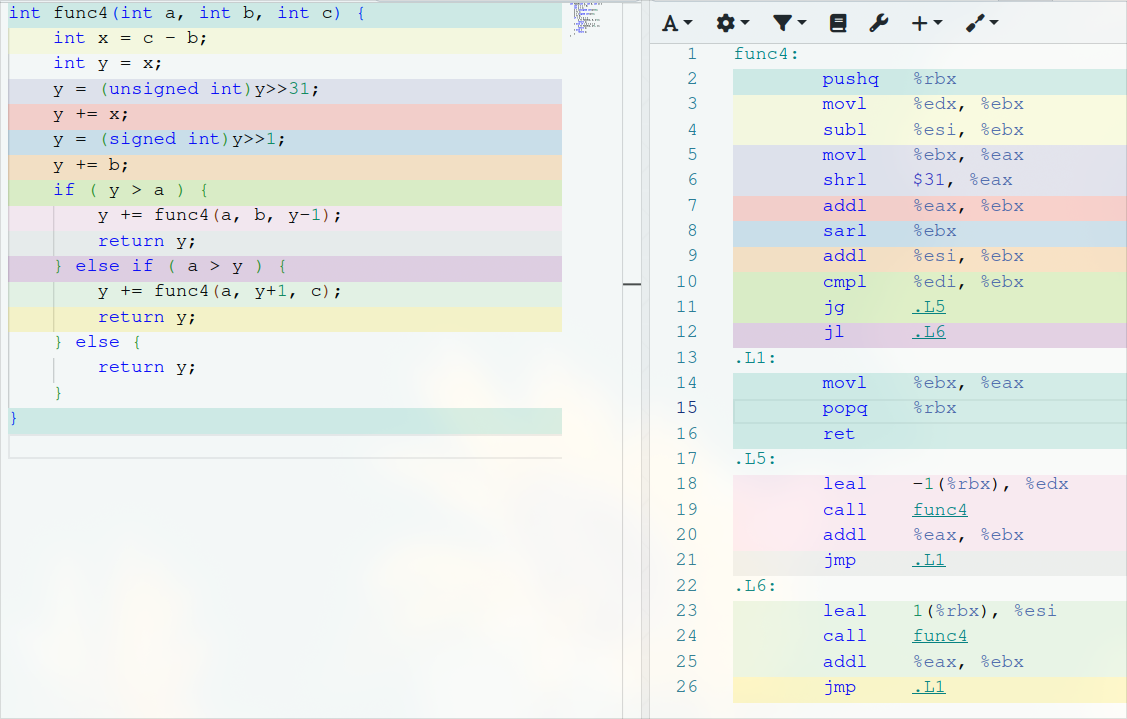
\includegraphics[scale=0.28]{func4.png}
	\end{center}
	Ég lenti í miklum vandræðum hér þar sem hvað sem ég reyndi gaf fallið ekki 
	niðurstöðuna 25 þangað til ég fattaði að ég var að leita að 0x25 ekki 
	bara 25, sem er þá í decimal 37 og þá gefur inntakið 10 þá útkomu. Svo 
	sést augljóslega að seinni talan á að vera $37$ og þá er lausnin komin, 
	"10 37".

	\section{}
	Um leið sést að inntaksstrengurinn þarf að vera af lengd $6$. Síðan er 
	lykkja sem fer í gegn um öll bæti strengsins og AND-ar þau við 0xf, sem 
	tekur í raun bara hægri hex stafinn í bætinu. Svo er það gildi notað 
	til að fá eitthvað gildi í minni sem er falið og það gildi bætt við 
	lokaniðurstöðu sem á að vera jöfn 0x25 eða 37 í endann. Ég byrjaði þá 
	á því að athuga öll mögulegu óþekktu gildin í minninu með því að nota 
	gdb til að athuga alltaf á minni í $\%rsi + 4i$ eftir þessa skipun 
	(ég lærði loksins hvernig á að breaka á sérstökum skipunum)
	\begin{center}
		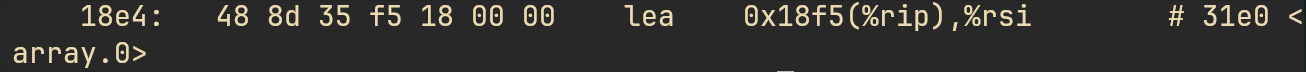
\includegraphics[scale=0.35]{rsi.png}
	\end{center}
	Og þá kemur út: 0x07, 0x03, 0x0a, 0x04, 0x10, 0x09, 0x0b, 0x08, 0x0c, 
	0x0f, 0x0d, 0x06.

	Ég nýti mér þá þetta til að ákveða að ég vil 0x03 þrisvar, 0x06 einu 
	sinni, 0x0a einu sinni og loks 0x0c. Til þess nota ég strenginn 
	"111;28".

	\section{}

	Hér er almennt þema á hvernig ég leysti þetta. Ég fattaði að magn kóða í 
	þessu falli er svolítið mikið svo ég ákvað að sleppa því að reyna að 
	afkóða nákvæmlega hvað fallið gerir og í staðinn finna hvernig hvert 
	inntak sem ég setti inn breytti stöðu fallsins og nota það til að 
	komast framhjá öllum köllum á explode\_bomb. Svo ég sé náttúrulega 
	fyrst að þetta eru 6 tölur og aðeins seinna í kóðanum er tölunum 
	rennt í gegn um lykkju sem athugar hvort þær séu allar á bilinu 1-6 og 
	hvort þær séu allar ólíkar.
	\begin{center}
		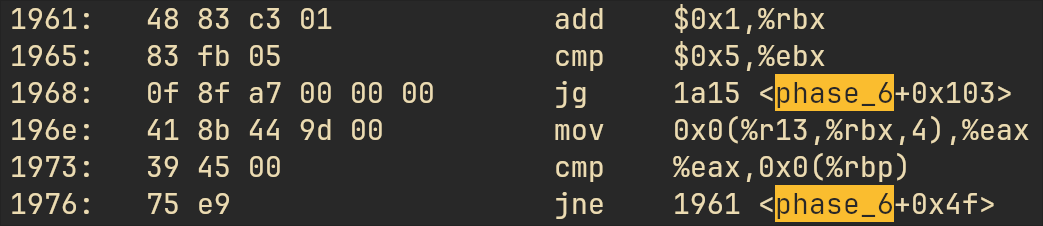
\includegraphics[scale=0.35]{1961.png}
	\end{center}
	\begin{center}
		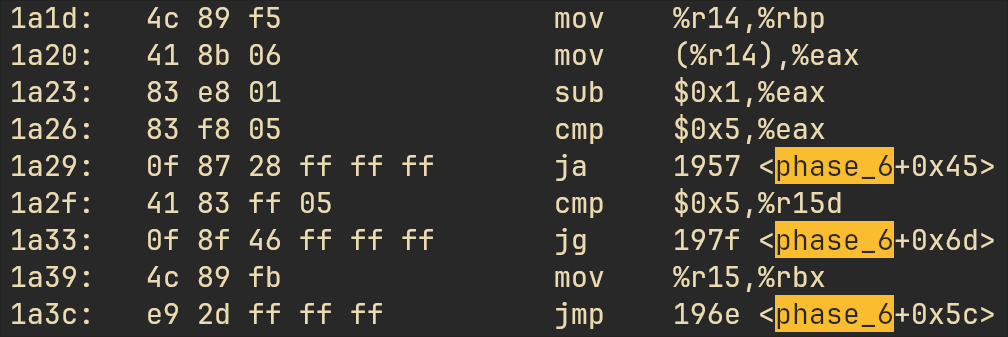
\includegraphics[scale=0.35]{1a1d.png}
	\end{center}

	Síðan er rennt í gegn um heilmikið magn reikninga og ég gat séð 
	nokkurnveginn útfrá þessu að við tökum inntakstölurnar og drögum þær 
	allar frá $7$ svo þær snúast í raun við. Síðan er rennt í gegn um kóða sem mér sýnist 
	setja einhver gildi falin í minni inn í stað gildanna sem voru lesin með 
	read\_six\_numbers og hér nennti ég eiginlega ekki að lesa úr öllum þessum 
	reikningum þannig að ég athugaði hvar var næst kallað á explode\_bomb. 
	\begin{center}
		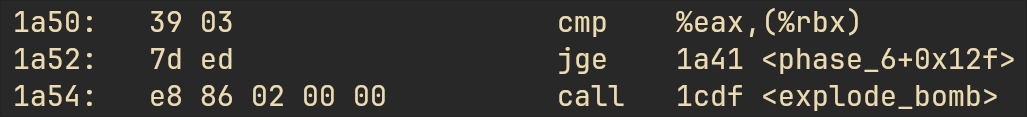
\includegraphics[scale=0.35]{cmp.png}
	\end{center}
	Frá þessu gat ég athugað með því að breyta inntakinu mínu á mismunandi hátt 
	að verið var að bera saman gildin í minni sem fyrstu tvær tölurnar leiddu til. 
	Með þessu gat ég athugað á gistunum og tékkað hvaða gildi þetta voru. Ég gerði 
	þetta þá fyrst með 1 2 sem fyrstu tölurnar, síðan 3 4 og loks 5 6. Ég var þá 
	kominn með lista yfir hvert gildi sem hver tala leiddi til.
	\[1 = 0x33e\]
	\[2 = 0x34f\]
	\[3 = 0x2c0\]
	\[4 = 0x352\]
	\[5 = 0x3cb\]
	\[6 = 0x299\]
	Eftir það er augljóst að sjá að forritið ber saman tölu 1 og tölu 2 og heldur 
	áfram ef tala 1 er stærri en tala 2, svo fer það í 2 og 3 o.s.frv. svo gildin 
	eiga að vera í lækkandi stærðarröð. Auðvelt er þá að raða þeim í svoleiðis röð 
	og fæst út talnarunan 5 4 2 1 3 6.


\end{document}
